\documentclass{article}
\usepackage[utf8]{inputenc}
 \usepackage{enumerate}
 \usepackage[T1]{fontenc}
\usepackage{cite}
%\usepackage{caption}
%\usepackage{subcaption}
\usepackage{mathtools}
\usepackage{stackengine}
\def\delequal{\mathrel{\ensurestackMath{\stackon[1pt]{=}{\scriptstyle\Delta}}}}
\usepackage{amsmath,amssymb,amsfonts}
\usepackage{amsmath,epsfig,cite,amsfonts,amssymb,psfrag,subfigure}
\usepackage{graphicx}
\usepackage{blindtext}
\usepackage{textcomp}
\usepackage{xcolor}
\usepackage{algorithm}
\usepackage[noend]{algpseudocode}
\usepackage{amsthm}
\def\BibTeX{{\rm B\kern-.05em{\sc i\kern-.025em b}\kern-.08em
    T\kern-.1667em\lower.7ex\hbox{E}\kern-.125emX}}
\allowdisplaybreaks
\newtheorem{remark}{Remark}
\newtheorem{theorem}{Theorem}
\newtheorem{lemma}{Lemma}
\newtheorem{proposition}{Proposition}
\newtheorem{corollary}{Corollary}
\newcommand{\diag}{\mathop{\mathrm{diag}}}
\DeclareMathOperator{\E}{\mathbb{E}}
\usepackage[margin=0.7in]{geometry}
\usepackage[export]{adjustbox}

\title{Reporte de inventario de eviencias}
\author{Natalia Galeano Valerio}
\date{Octubre 2019}

\begin{document}


\baselineskip 12pt

\vspace*{30mm}

\begin{center}

\textbf{\Large Research Plan} \\
\vspace{10mm}
\textbf{Department of Electrical and Computer Engineering}\\
\vspace{20mm}
%{\large University of Oulu}\\
{\large University of Tehran}\\
\vspace{20mm}
\end{center}
\vspace{10mm}
{\scriptsize Provisional title:}\\
Dynamic Resource Allocation in O-RAN Architecture using Network Slicing\\

\vspace{20mm}

{\scriptsize Candidate name}\\
Mojdeh Karbalaee Motalleb \\
\vspace{3mm}



%{\scriptsize Supervisor name:}\\
%Dr. Onel Lopez\\
\vspace{3mm}


\pagebreak
\begin{abstract}
Open radio access network (O-RAN) is the next generation of RAN systems introduced by the O-RAN Alliance to increase the flexibility and the openness of the network systems and simultaneously decrease CAPEX and OPEX of mobile operators. The O-RAN system combines and takes advantage of Cloud RAN (C-RAN) and the Virtual RAN (VRAN).
O-RAN separates RAN into three
different units, namely Radio Unit (O-RU), Distributed Unit
(O-DU), and Central Unit (O-CU).
In this research, we study
the problem of baseband resource allocation and virtual
network function (VNF) activation in O-RAN architecture
based on their service priority for different types of 5G services
including enhanced mobile broadband (eMBB), ultra-reliable
low latency communications (uRLLC) and massive Machine
Type Communications (mMTC) services using intelligent RAN slicing. 
Network slicing is a promising solution for supporting such heterogeneous and challenging services.
Deploying network slicing, the isolation of different types of services in O-DU, O-CU, and user plane function (UPF) is performed. The limited
fronthaul capacity, the restriction of end-to-end delay and the reliability of the services are
considered at the same time.
The optimization of baseband
resources includes O-RU assignment, the assignment of physical resource blocks
(PRBs), and power allocation. The main problem is a mixed-integer non-linear programming problem that is tremendously difficult. Since the problem has a two-time scale, it can be broken into two layers. On the large-time scale, the problem of obtaining the optimal number of VNF, the placement of VNFs, and the assignment of PRB to the slices are considered. 
On the small-time scale, there is a problem of obtaining the optimal power of UEs, and the PRB and O-RU assignment.
To solve the problem, we propose deep reinforcement learning, the deep deterministic policy gradient (DDPG) method, and convex optimization.
\end{abstract}
\section{Introduction} 
Open radio access network (O-RAN), as the integration and expansion of cloud RAN (C-RAN) and xRAN, or C-RAN and virtual RAN (vRAN), is expected to be a key technology in 5G networks to enhance the RAN performance extensively. 
The core idea of C-RAN is to divide the radio remote head (RRU) from the baseband unit (BBU). Also, several BBUs are placed together to create the BBU-pool, providing unified baseband signal processing with powerful computing capabilities. On the other hand, xRAN technology has three fundamental features. The control plane is decoupled from the user plane. Besides, a modular eNB software stack is built to operate on common-off-the-shelf (COTS) hardware. Moreover, open north-bound and south-bound interfaces are introduced.
O-RAN, as illustrated in Fig. \ref{fig:c11}, separates RAN into three different units, namely Radio Unit (O-RU), Distributed Unit (O-DU), and Central Unit (O-CU). O-RU is a logical node that contains RF and lowers PHY. Moreover, the O-DU expresses another logical node that includes higher PHY, MAC, and RLC. In addition, the O-CU depicts the logical node contains two parts: the O-CU user plane (O-CU-UP) and O-CU control plane (O-CU-CP). O-CU-UP hosts PDCP-UP and SDAP, and O-CU-CP hosts PDCP-CP and RRC. O-DU and O-CU are connected via an open and well-defined interface F1.
Moreover, O-DU is connected to a radio unit (O-RU) with an open fronthaul interface.
The architecture of O-RAN contains other principal logical nodes called Orchestration and Automation,
RAN Intelligent Controller (RIC)- Near Real-Time and O-Cloud. 
One of the necessities of the new generation of wireless networks is its intelligence.
Based on the requirement of an intelligent wireless network, O-RAN offers machine learning techniques. The two logical nodes RIC-Non Real-Time (which is placed in Orchestration and Automation node) and RIC- Near Real-Time, implement the algorithms for network intelligence
\cite{gavrilovska2020cloud,niknam2020intelligent,kazemifard2021minimum,both2021system,ORANArch,ORANML,lin2021toward}.
\begin{figure*}
  \centering 
    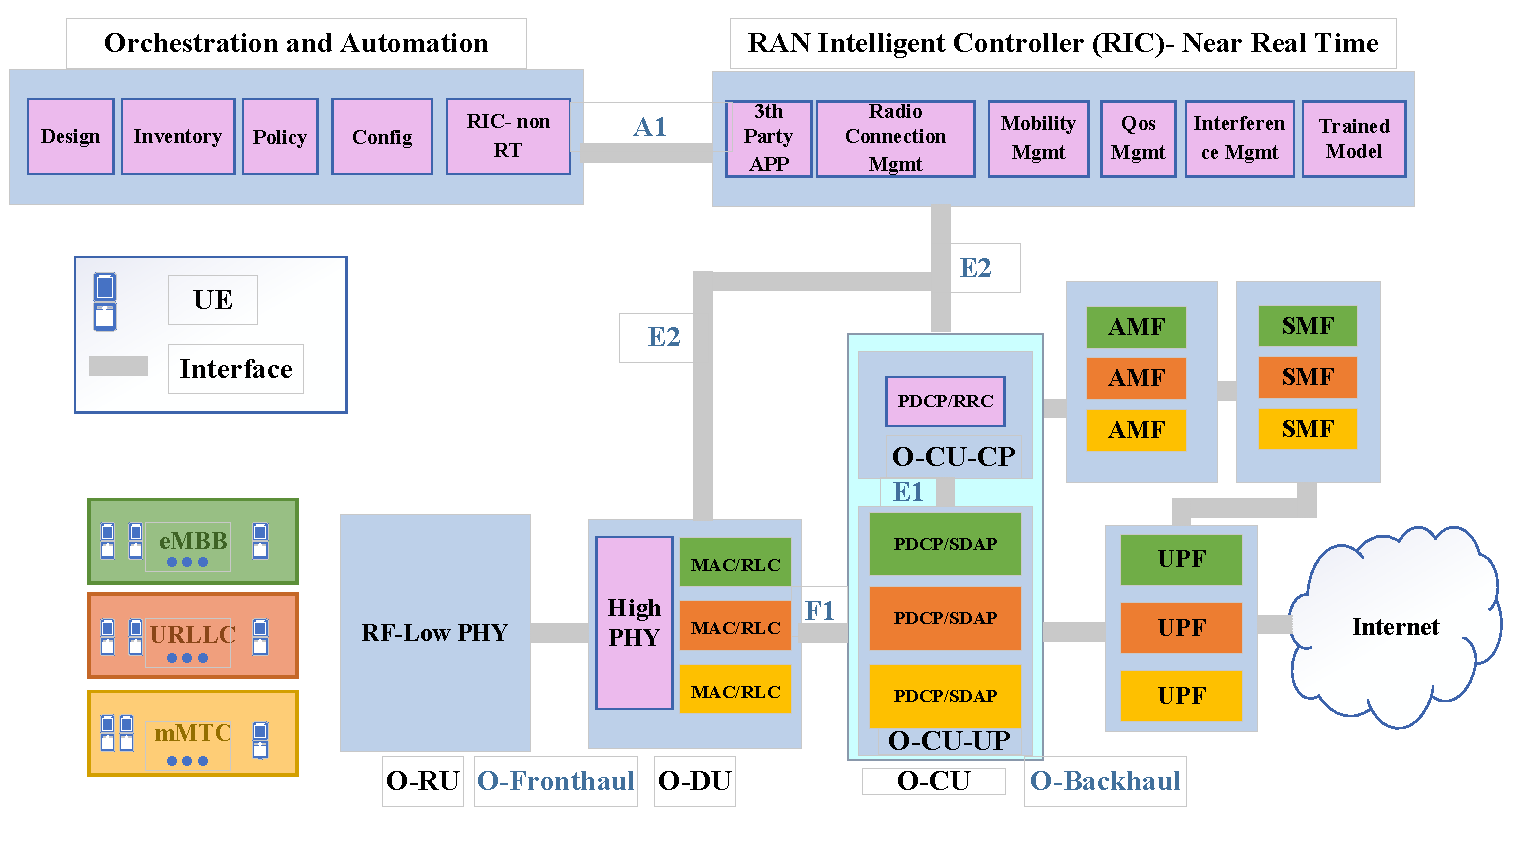
\includegraphics[scale = 0.5]{finalDraw.pdf}
    %\includegraphics[max height=30cm,max width=9.5cm]{Drawing15.eps}
    %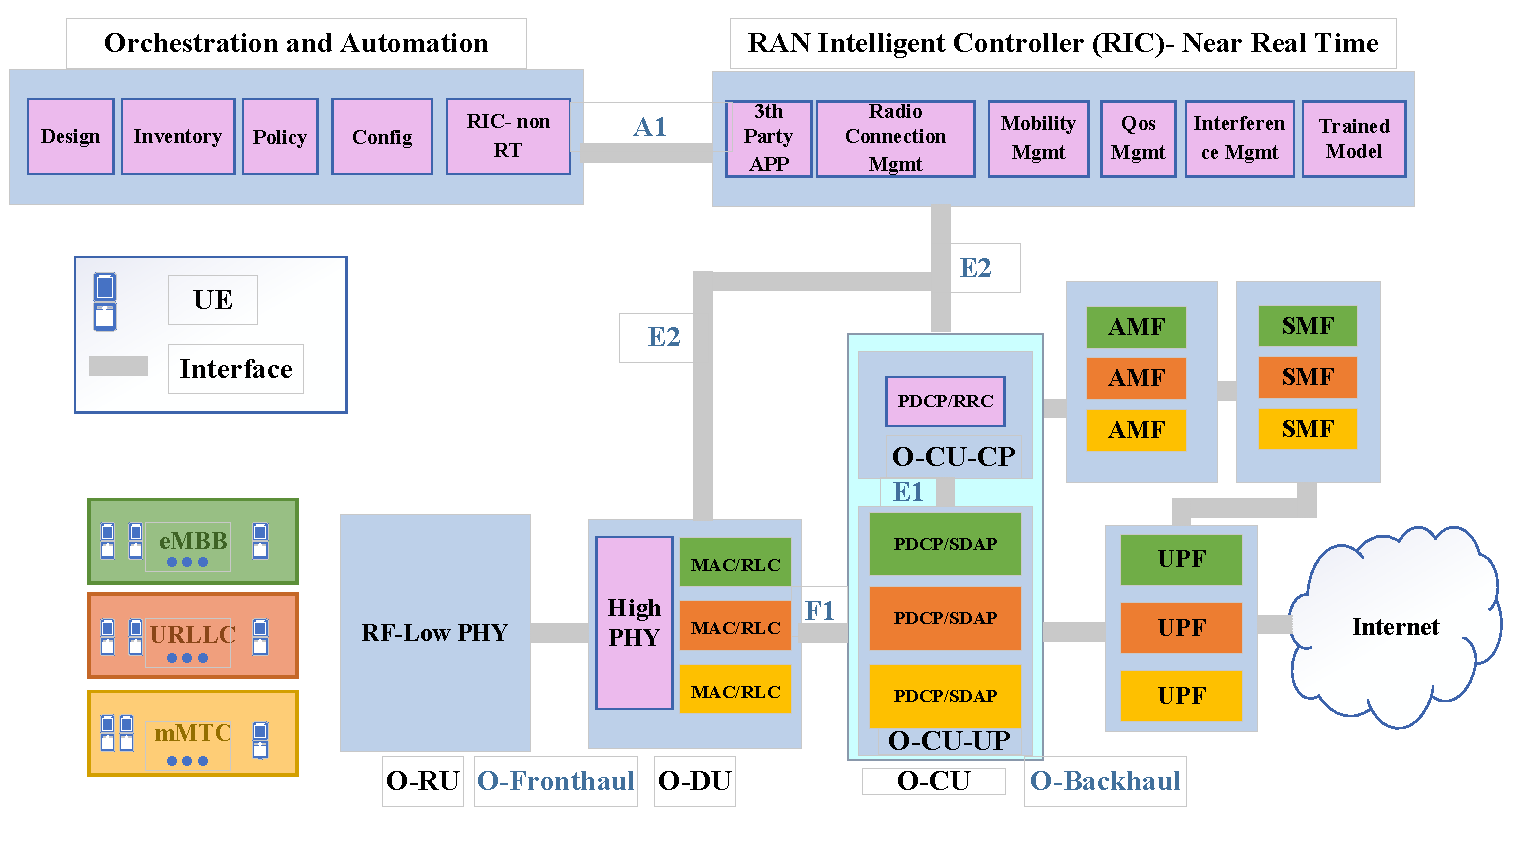
\includegraphics[width=\textwidth]{finalDraw.pdf}
  \caption{Network sliced ORAN system}
  \label{fig:c11}
\end{figure*}


One of the goals of the next generation of mobile systems is to strictly meet the stringent QoS demands of the different services introduced in 5G , i.e., eMBB, URLLC, and mMTC. Network slicing is a promising solution to obtain the QoS for each type of service. Network slicing contains RAN slicing, core slicing, and both of them together. Efficient slicing of RAN is still challenging due to time-varying network circumstances.
%Network slicing will propose significant complexity into the performance of systems that causes conventional mathematical model-based procedures to network operation no longer adequate. 
Network slicing creates considerable complexity in system performance and makes the conventional mathematical methods insufficient to model the network.
Therefore, it motivates researchers to realize network slicing using machine learning strategies such as deep learning and deep reinforcement learning. So, the network can reach the best control policy according to its experience in the past time slots.
As mentioned above, network slicing, which contains RAN slicing, core slicing, and the whole, is considered a hot topic for vendors. In addition, the O-RAN system seems to be the next RAN architecture. So, this motivated researchers to study the dynamic RAN slicing in O-RAN architecture to achieve the desired QoS for each service type.
In addition, according to the high complexity of RAN slicing and incapability of the traditional model-based methods, dynamic machine learning becomes the best solution for these problems.
 Generally, there are two kinds of deep reinforcement learning methods for solving dynamic problems. The first class is value-based such as Deep-Q-Network, and the second class is policy-based problems such as
deep deterministic policy gradient (DDPG). The first class can only solve the discrete action space problems, which are integer programming. The second class can solve by searching the optimal policy, which is the actor-critic method. Here, we use the second method to solve our problems \cite{alsenwi2021intelligent,yan2019intelligent,mei2021intelligent}.
\subsection{Related Works} 
In \cite{mei2021intelligent}, the authors proposes a new intelligent RAN slicing method with two-layered control granularity, which aims at maximizing both the long-term QoS of services and spectrum efficiency (SE) of slices. In this paper, the authors design a RAN slicing strategy with multiple time and
resource granularities to accommodate the time-varying network conditions and diverse QoS requirements.
Here, the DDPG method is applied for the lower level and deep Q-network is applied for upper level.
In paper \cite{rezazadeh2021actor}, an actor-critic methods and a continuous model-free deep reinforcement
learning (DRL) method is applied to minimize energy consumption and virtual network function (VNF) instantiation cost.
Multiplexing eMBB and uRLLC services on the same RAN and sharing the resources of these services is challenging, and many researchers pay attention to this issue.
In \cite{setayesh2020joint,yang2020should}, the problem of resource allocation in the coexistence of URLLC and eMBB services is considered based on their QoS. 
Paper \cite{alsenwi2021intelligent}, represents a joint convex method and deep reinforcement learning to schedule both eMBB and URLLC services. Here we have two time-scale, a two-phase-framework, including eMBB resource allocation and URLLC scheduling phases.  
In \cite{saggese2021power}, the problem of power minimization for uRLLC and eMBB services is presented for non-orthogonal multiple access (NOMA) and orthogonal multiple access (OMA).
 In \cite{korrai2020ran}, the authors proposed to allocate RAN resources for the network slicing system in coexistence of eMBB and URLLC services. The system guarantees the latency, the service rate, and the maintenance of reliability.

\subsection{Main Contributions}
In this research, as depicted in Figure \ref{fig:c11}, we aim at solving the problem of dynamic network slicing in the O-RAN system. 
Here, we study a single-cell downlink situation involving multiple network slices that share existing radio sources.
The main contributions of
this research are summarized as follow:
\begin{itemize}
\item 
Here, we separate the scheduling into two-time scales. So we considered the two-time scale system and solved it in two layers. On a large time scale, the problem of obtaining an optimal number of VNFs and the VNF placement is performed. Also, the assignment of PRB to the slices is obtained. On a small-time scale, the problem of power allocation, O-RU association, and the assignment of PRB to UE in each slice is applied.
\item 
We consider three types of services that requires specific QoS: i) URLLC, which requires low latency and high reliability; ii) eMBB, which needs high data rate; and iii) mMTC, which demand short-packet connectivity support for a massive number of low-power devices.
The problem of RAN slicing for different types of services is studied in this research.

\item 
We consider an intelligent resource allocation in the O-RAN architecture for the different services. Since conventional models do not perform well here because of the heterogeneous QoS requirements of each service type and the complexity of dynamic RAN slicing. So we must switch to machine learning and dynamic methods and find the most suitable approach.  
A dynamic strategy of resource allocation is required to solve this problem to achieve the specific QoS for each type of service in the O-RAN architecture.
 In the small-time scale, the actor-critic algorithm such as DDPG is applied to the system that is based on control policy search. This method directly searches the optimal control policy
by estimating of the gradient with respect to the parameters
of the control policy. In the large-time scale, the deep Q-Network is implemented which is a value based algorithm and it can find best solution for discrete action-state.
\item 
We aim to apply transfer learning to the system and study the enhancement of performance and convergence. We can use Q-value transfer learning and action-selection transfer learning, So agents can utilize the knowledge of experts to improve their performance on current tasks\cite{zhou2021learning}. 
\end{itemize}
\section{Current State of the Research}
\subsection{System Model}
Assume we have $S$ preallocated slices serving $S$ services contains eMBB, URLLC, and mMTC services; There are $S_1$ slices for the first service type (eMBB), $S_2$ slices for the second service type (URLLC), and $S_3$ slices for the third service type (mMTC), , thus $S=S_1+S_2+S_3$.
Each Service $s\in \{1,2,...,S\} $ consists of $U_{s}$ single-antenna user equipments (UEs) which require certain QoS to be able to use the requested program.
There are different application requests which fall into one of these service categories. Each application request requires specific QoS. Based on the request for the application and QoS, a UE may be admitted and allocated to the resources.
Assume each slice $s \in \{1,2,...,S \}$, consists of $K_{s}$, pre-allocated physical resource blocks (PRBs)  obtained in the large-time scale, $M_s^{d}$ VNFs for the processing of O-DU, $M_s^{c}$ VNFs for the processing of O-CU-UP and $M_s^{u}$ VNFs for the processing of UPF. 
Virtual network functions (VNFs) are functional blocks of the
system. Each VNF instance is running on a virtual machine (VM) using resources from the data centers. Each VM, requires enough resources of CPU, memory, storage and network bandwidth.

In addition, there are $R$ multi-antenna RU that are shared between slices. Each RU $r \in \{1,2,...,R \}$
has $J$ antenna for transmitting and receiving data. Moreover, all RUs, have access to PRBs.
\subsection{The Achievable Rate}
The SNR of $i^{th}$ UE requesting served at slice $s$ on PRB $k$ is obtained from
\begin{equation}\label{eq2}
\rho_{r,u(s,i)}^{k} =  \frac{|p_{r,u(s,i)}^{k}{\bold{h}_{r,u(s,i)}^{H \: k}} \bold{w}_{r,u(s,i)}^{k}|^2}{BN_0 + I_{r,u(s,i)}^{k}},
\end{equation} 
where $p_{r,u(s,i)}^{k}$ represents the transmission power from O-RU $r$ to $i^{th}$ UE served at slice $s$ on PRB $k$. 
${\bold{h}_{r,u(s,i)}^{k}} \in \mathbb{C}^{J}$ is the vector of channel gain of a wireless link from 
$r^{th}$ RU to the $i^{th}$ UE in $s^{th}$ slice. In addition, $\bold{w}_{r,u(s,i)}^{k} \in \mathbb{C}^{J}$ depicts the  transmit beamforming vector from $r^{th}$ RU to the $i^{th}$ UE in $s^{th}$ slice that is the zero forcing beamforming vector to minimize the interference which is indicated as below
\begin{equation}
\bold{w}_{r,u(s,i)}^{k} = {\bold{h}_{r,u(s,i)}^{k}}({\bold{h}_{r,u(s,i)}^{H \: k}} {\bold{h}_{r,u(s,i)}^{k}})^{-1}.
\end{equation}
Moreover, $g_{u(s,i)}^r \in \{0,1\}$ is a binary variable that illustrates whether RU $r$ is mapped to the $i^{th}$ UE allocated to $s^{th}$ slice or not. 
Also, $BN_0$ denotes the power of Gaussian additive noise, and $I_{r,u(s,i)}^{k}$ is the power of interfering signals represented as follow
\begin{equation}\label{eqI}
\begin{split}
I_{r,u(s,i)}^{k} &=
 \underbrace{\sum_{\substack{l=1 \\ l\neq i}}^{{U}_{s}} \gamma_{1}  p_{u(s,l)}^{k}\sum_{\substack{r'=1 \\ r'\neq r}}^{R}|{\bold{h}_{r',u(s,i)}^{H \: k}} \bold{w}_{r',u(s,l)}^{k} g_{u(s,l)}^{r'}|^2}_{\text{(intra-slice interference)}}\\
&+ \underbrace{\sum_{\substack{n = 1 \\ n\neq s}}^{S}\sum_{l=1}^{{U}_s} \gamma_{2}  p_{u(n,l)}^{k}\sum_{\substack{r'=1 \\ r'\neq r}}^{R}|{\bold{h}_{r',u(s,i)}^{H \: k}} \bold{w}_{r',u(n,l)}^{k} g_{u(n,l)}^{r'}|^2}_{\text{(inter-slice interference)}}\\
&+\underbrace{  \sum_{j=1}^{{R}} {\sigma_q}^2 |\boldsymbol{h}_{r,{u(s,i)}}^k|^2 }_{\text{(quantization noise)}},
\end{split}
\end{equation}
where $\gamma_{1} = e^{k}_{u(s,i)}e^{k}_{u(s,l)}$ and $\gamma_{2} = e^{k}_{u(s,i)}e^{k}_{u(n,l)}$.
$e^{k}_{u(s,i)}$ is the binary variable to show whether the $k^{th}$ PRB is allocated to the UE $i$ in slice $s$, assigned to $r^{th}$ O-RU.

The achievable data rate for the $i^{th}$ UE request in the $s_{1}^{th}$ application of service type 1 (eMBB) can be written as $\mathcal{R}_{u(s_1,i)}^{e}$.
\begin{equation}\label{eq1}
\begin{split}
\mathcal{R}_{u(s_1,i)}^{e,r} &= \sum_{k=1}^{K_{s_1}} B \log_2({1+ \rho_{r,u(s_1,i)}^{k}})a_{u(s_1,i)} e^k_{r,u(s_1,i)},\\
\mathcal{R}_{u(s_1,i)}^{e} &= \sum_{r=1}^{R}\mathcal{R}_{u(s_1,i)}^{e,r},
\end{split}
\end{equation}
where $B$ is the bandwidth of system. 
$\mathcal{R}_{u(s_1,i)}^{e,r}$ is the achievable rate of each RU $r$ to UE $i$ in slice $s_1$.
Since the blocklength in URLLC and mMTC is finite, the achievable data rate for the $i^{th}$ UE request in the $s_{j}^{th} $, $j \in \{2,3\}$ application of service type 2 (URLLC) and 3 (mMTC) is not achieved from Shannon Capacity formula. So, for the short packet transmission the achievable data rate is approximated as follow
\begin{equation}\label{eq11}
\begin{split}
\mathcal{R}_{u(s_2,i)}^{\mathfrak{u},r} &= \sum_{k=1}^{K_{s_2}} B (\log_2({1+ \rho_{u(s_2,i)}^{k}})- \zeta_{u(s_2,i)}^{k}){\beta}_{u(s_2,i)}^{k}, \quad \mathfrak{u} \in  \{u,m\}, \\
\mathcal{R}_{u(s_1,i)}^{\mathfrak{u}} &= \sum_{r=1}^{R}\mathcal{R}_{u(s_2,i)}^{e,r}, 
\end{split}
\end{equation}
where ${\beta}_{u(s_2,i)}^{k}=a_{u(s_2,i)} e^{k}_{u(s_2,i)}$
and $\zeta_{u(s_2,i)}^{k} = \log_2({e})Q^{-1}(\epsilon) \sqrt{\frac{C_{u(s_2,i)}^{k}}{N_{u(s_2,i)}^{k}}})$
where $\epsilon$ is the transmission error probability, $Q^{-1}$ is the inverse of Q function (i.e., Gaussian),
$C_{u(s_2,i)}^{k} = 1 - \frac{1}{(1+\rho_{u(s_2,i)}^{k})^2}$ depicts the channel dispersion of UE  $i$ at slice $s_2$, experiencing PRB $k$ and
$N_{u(s_2,i)}^{k}$ represents the blocklength of it. 
$\mathcal{R}_{u(s_1,i)}^{e,r}$ is the achievable rate of each RU $r$ to UE $i$ in slice $s_2$.
\subsection{Mean Delay}
In this part, the end-to-end mean delay for each service is obtained.
Suppose the mean total delay is depicted as $T_{\text{\text{tot}}}$,
\begin{equation}
\begin{split}
T^{\text{\text{tot}}} &=  T^{\text{proc}} + T^{tr} + T^{\text{pro}},\\
T^{\text{\text{proc}}} &=  T^{RU} + T^{DU} + T^{CU} + T^{UPF},\\
T^{tr} &= T^{fr,t} + T^{\text{mid},t} + T^{b,t},  \\
T^{\text{pro}} &= T^{fr,p} + T^{\text{mid},p} + T^{b,p}.  \\
\end{split}
\end{equation}
%{\color{red} I made a mistake and replaced pro with proc. Please correct them. Also, explain in more details the processing delay in this paragraph.}
%T_{\text{\text{tot}}} = T_{RU} + T_{front} + T_{DU} + T_{\text{mid}} + T_{CU} + T_{back} + T_{core} + T_{trans2net}
The total delay ($T^{\text{\text{tot}}}$), is the sum of the processing delay ($T^{\text{proc}}$), the transmission delay ($T^{tr}$), and the propagation delay ($T^{\text{pro}}$). 
The propagation delay is the time takes for a signal to reach its destination. It obtains based on the length of the fiber link and the capacity of the link ($T = L/c$, where $L$ is the length of the link and c is the capacity of the link). The total propagation delay ($T^{\text{pro}}$), is the sum of the propagation delay in the fronthaul link $T^{fr,p}$, the midhaul link $T^{\text{mid},p}$, and the backhaul link $T^{b,p}$.
Also, the transmission delay is the amount of time required to push all the packets into the fiber link.
Moreover, it can formulated as 
$T = \frac{\mathcal{\alpha}}{R}$, where $R$ is the sum-rate of the packet transmission in each link and $\mathcal{\alpha}$ is the mean arrival data rate of each link.
So the total transmission delay ($T^{tr}$) is the sum of the transmission delay in the fronthaul $T^{fr,t}$, the midhaul $T^{\text{mid},t}$, and the backhaul $T^{b,t}$.
In this paper, we focus only on the processing delays to find the optimal number of VNFs, and we ignore the other two delays for simplification;
So, we assume that the total delay is approximate to the processing delay, i.e.,
%Here we assume the propagation delay and the transmission delay are negligible compared to the processing delay.
\begin{equation}
T^{\text{\text{tot}}} \approx T^{\text{proc}}.
\end{equation}
\subsubsection{Processing Delay}
Assume the packet arrival of UEs follows a Poisson process with arrival rate $\lambda_{u(s,i)}$ for the $i^{th}$ UE of the $s^{th}$ service (or slice).
Therefore, the mean arrival data rate of the $s^{th}$ slice in the UPF layer is $\alpha_{s}^U = \sum_{u=1}^{U_s}\lambda_{u(s,i)}$.
Assume the mean arrival data rate of the UPF layer for slice $s$ ($\alpha_{s}^U$) is approximately equal to the mean arrival data rate of the O-CU-UP layer ($\alpha_{s}^C$) and the O-DU ($\alpha_{s}^D$). so $\alpha_{s} =\alpha_{s}^U \approx \alpha_{s}^C \approx \alpha_{s}^D$,
Because the amount of data traffic transferred along the route (regardless of frame changes) is constant.
Since, by using Burke’s theorem, the mean arrival data rate of the second and third layers, which are processed in the first layer, is still poisson with rate $\alpha_{s}$.
It is assumed that there are load balancers in each layer for each service to divide the incoming traffic to VNFs equally. %\cite{frdl,luong2018novel,luong2018novel1}.
Suppose the baseband processing of each VNF is depicted as M/M/1 processing queue.
Each packet is processed by one of the VNFs of a slice. So, the mean delay for the $s^{th}$ slice in the O-DU, the O-CU, and the UPF is modeled as M/M/1 queue, is formulated as follows, respectively \cite{SystemCostMinimization,luong2018joint,luong2018novel},
\begin{equation}
\begin{split}
T_{s}^{DU} &= \frac{1}{\mu_s^d - \alpha_{s}/{M_s^{d}}},\\
T_{s}^{CU} &= \frac{1}{\mu_s^c - \alpha_{s}/{M_s^{c}}},\\
T_{s}^{UPF} &= \frac{1}{\mu_s^u - \alpha_{s}/{M_s^{u}}},\\
\end{split}
\end{equation}
where $M_s^{d}$, $M_s^{c}$ and 
$M_s^{u}$ are the variables that depict the number of VNFs in O-DU, O-CU-UP and UPF, respectively. 
Moreover, $1/\mu_s^d$, $1/\mu_s^c$, and $1/\mu_s^u$ are the mean service time of the O-DU, O-CU, and the UPF layers, respectively.
Besides, $\alpha_{s}$ is the  arrival rate which is divided
by load balancer before arriving to the VNFs. The arrival rate of each VNF in each layer for each slice 
$s$ is $\alpha_{s}/{M_s^{i}}$ $ i \in \{d,c, u\}$.

$T_{u(s,i)}^{RU}$ is the mean transmission delay of the $i^{th}$ UE of the $s^{th}$ service on the wireless link.
 The arrival data rate of wireless link for each UE $i$ of service $s$ is $\lambda_{u(s,i)}$
As a result, we have $\sum_{i = 1}^{U_s} \lambda_{u(s,i)} = \alpha_s$.
Moreover, The service time of transmission queue for UE $i$ requesting service $s$ has
an exponential distribution with mean $1/R_{u(s,i)}$ and can be modeled as a M/M/1 queue \cite{SystemCostMinimization,luong2018joint,luong2018novel}.
 
Therefore, the mean delay of the transmission layer for UE $i$ in slice $s$ is
\begin{equation}
 T_{u(s,i)}^{RU} = \frac{1}{R_{u(s,i)} - \lambda_{u(s,i)}}.
\end{equation}

So, the mean processing delay for UE $i$ in slice $s$ is 
\begin{equation}
T^{\text{proc}}_{u(s,i)} =  T^{RU}_{u(s,i)} + T^{DU}_{s} + T^{CU}_{s} + T^{UPF}_{s}.
\end{equation}
Hence, for the simplification and focusing on the processing delay, we assume $T^{\text{\text{tot}}}_{u(s,i)} \approx T^{\text{proc}}_{u(s,i)} $.
%\subsection{Reliability of URLLC}
%As we know, UEs request URLLC services, require services with low latency.
%For the M/M/1 system, the probability of the delay for each application $s$ in the UPF, CU, DU and RU is as follow, respectively
%\begin{equation}
%\begin{split}
%P_r\{T_{UPF}^{s} \geq T_{UPF}^{max}\} &= e^{-(\mu_u - \alpha_{s}/{M_s^{u}})T_{UPF}^{max}}\\
%P_r\{T_{CU}^{s} \geq T_{CU}^{max}\} &= e^{-(\mu_c - \alpha_{s}/{M_s^{c}})T_{CU}^{max}}\\
%P_r\{T_{DU}^{s} \geq T_{DU}^{max}\} &= e^{-(\mu_d - \alpha_{s}/{M_s^{d}})T_{DU}^{max}}\\
%P_r\{T_{RU}^{s} \geq T_{RU}^{max}\} &= e^{-(R_{{tot}_s} - \alpha_{s})T_{RU}^{max}}\\
%\end{split}
%\end{equation} 
%So the probability of coincidence of these events is as follow
%\begin{equation}
%P_r\{E_1, E_2, E_3, E_4\} = A_1 A_2 A_3 A_4,
%\end{equation}
%where $E_1 = T_{UPF}^{s} \geq T_{UPF}^{max}$, $E_2 =T_{CU}^{s} \geq T_{CU}^{max} $, $E_3 =T_{DU}^{s} \geq T_{DU}^{max} $ and $E_4 =T_{RU}^{s} \geq T_{RU}^{max} $.
%Also $A_1=e^{-(\mu_u - \alpha_{s}/{M_s^{u}})T_{UPF}^{max}}$, $A_2=e^{-(\mu_c - \alpha_{s}/{M_s^{c}})T_{CU}^{max}}$, $A_3= e^{-(\mu_d - \alpha_{s}/{M_s^{d}})T_{DU}^{max}}$ and $A_4 = e^{-(R_{{tot}_s} - \alpha_{s})T_{RU}^{max}}$.
\subsection{Physical Data Center Resource}
Each VNF requires
physical resources that include memory, storage, CPU and Network Bandwidth.
Let the required resources for VNF $f$ in slice $s$ is represented by a tuple as
\begin{equation}
\bar{\Omega}_{s}^f = \{\Omega_{M,{s}}^f, \Omega_{S,{s}}^f, \Omega_{C,{s}}^f, \Omega_{N,{s}}^f \},
\end{equation}
where $\bar{\Omega}_{s}^f\in \mathbb{C}^{4}$ and $\Omega_{M,{s}}^f, \Omega_{S,{s}}^f, \Omega_{C,{s}}^f, \Omega_{N,{s}}^f$ indicate the amount of required memory, storage, CPU and and Network Bandwidth, respectively.
Moreover, the total amount of required memory, storage, CPU and Network Bandwidth of all VNFs of a slice in DU, CU and UPF is defined respectively as follows
\begin{equation}
\begin{split}
&\bar{\Omega}_{\mathfrak{z},s}^{tot,d} = \sum_{f=1}^{M_{s}^d}\bar{\Omega}_{\mathfrak{z},s}^{f,d},\\
&\bar{\Omega}_{\mathfrak{z},s}^{tot,c} = \sum_{f=1}^{M_{s}^c}\bar{\Omega}_{\mathfrak{z},s}^{f,c},\\
&\bar{\Omega}_{\mathfrak{z},s}^{tot,u} = \sum_{f=1}^{M_{s}^u}\bar{\Omega}_{\mathfrak{z},s}^{f,u}, \\
\end{split}
\end{equation}
$\forall \mathfrak{z} \in \{M, S, C, N\}$, where, $\bar{\Omega}_{\mathfrak{z},s}^{f,d}$, $\bar{\Omega}_{\mathfrak{z},s}^{f,c}$ and $\bar{\Omega}_{\mathfrak{z},s}^{f,u}$ are the amount of resource that a VNF required in DU, CU and UPF, respectively. Then,
\begin{equation}
 \bar{\Omega}_{\mathfrak{z},s}^{tot} = \bar{\Omega}_{\mathfrak{z},s}^{tot,d}+ \bar{\Omega}_{\mathfrak{z},s}^{tot,c}+\bar{\Omega}_{\mathfrak{z},s}^{tot,u}
\end{equation} 
Also, there are $D_c$ data centers (DC), serving the VNFs. Each DC contains several servers that supply VNF requirements.
The amount of memory, storage, CPU and and Network Bandwidth is denoted by $\tau_{M_{j}}, \tau_{S_{j}}$, $\tau_{C_{j}} $ and $\tau_{N_{j}} $ for the $j^{th}$ DC, respectively
\begin{equation*}
\tau_j = \{\tau_{M_{j}}, \tau_{S_{j}}, \tau_{C_{j}}, \tau_{N_{j}} \},
\end{equation*}
In this system model, the assignment of physical DC resources to VNFs is considered. Let $y_{s,d}$ be a binary variable indicating whether the $d^{th}$ DC is allocated the resources to the VNFs of $s^{th}$ slice or not.
\subsection{Power of the O-RU and the Fronthaul Capacity}
Let $P_r$ denote the power of the transmitted signal from the $r^{th}$ O-RU to UEs served by it. We have,
\begin{equation}\label{pr}
P_r = \sum_{s=1}^{S}\sum_{k=1}^{K_s}\sum_{i=1}^{U_s}|\bold{w}_{r,u(s,i)}^{k}|^2 p_{r,u(s,i)}^{k} g_{u(s,i)}^r e^k_{r,u(s,i)}+ \sigma_{q}^2.
\end{equation}
Since we have a fiber link between O-RU and O-DU, the rate of users on the fronthual link between O-DU and the $r^{th}$ O-RU  is formulated as
%\cite{simeone2016cloud, 1111}
\begin{equation}\label{cr}
C_{r} = \log{\left(1+ \frac{\sum_{s=1}^{S}\sum_{k=1}^{K_s}\sum_{i=1}^{U_s}|\bold{w}_{r,u(s,i)}^{k}|^2 \mathcal{\alpha}^k_{r,u(s,i)} }{ \sigma_{q}^2}\right)},
\end{equation}
where $\mathcal{\alpha}^k_{r,u(s,i)}= p_{r,u(s,i)}^{k} g_{u(s,i)}^r e^k_{r,u(s,i)}$ and $\sigma_{q}^2$ is the power of quantization noise.
\subsection{Problem Statement}
%In this system, the goal is to minimize the cost of the system.
%The total power cost of O-RUs for transmitting data to UE is depicted as follow
%\begin{equation}
%P_{tot} = \sum_{r=1}^{R}P_r
%\end{equation}
Assume the power consumption of baseband processing at each DC $d$ that is connected to VNFs of a slice $s$ is depicted as
$\phi_{s}$. So the total power of the system for all active DCs that are connected to slices can be represented as
\begin{equation*}
\textstyle \phi_{tot} = \sum_{s=1}^{S}\phi_{s} + \sum_{d=1}^{D_c}z_d \psi_d .
\end{equation*}
where, $z_d$ is shown that whether the $d^{th}$ DC is active or not and $\psi_d$ is a static cost when a DC is active, i.e.,
\begin{equation}
  z_d =
    \begin{cases}
      1 & \sum_{s=1}^{S}y_{s,d} \geq 1 \\
      0 & \text{otherwise}
    \end{cases}.       
\end{equation}  
Here, we assume that if any VNF placed in a server $d$ is used, the server is on and active, otherwise, it is off.
In addition, $\phi_{s}$ is obtained from below
\begin{equation}
\phi_{s} = M_s^u \phi_s^u + M_s^c \phi_s^c+ M_s^d \phi_s^d,
\end{equation}
where, $\phi_s^u$, $\phi_s^c$ and $\phi_s^d$ are the static cost of energy in UPF, CU and DU, respectively.
Here, we want to maximize the energy efficiency $\eta$. 
So the optimization problem is formulated as follow

\begin{subequations} \label{mainP}
\begin{alignat}{4}
\max\limits_{ \boldsymbol{M}, \boldsymbol{Y}, \boldsymbol{E},\boldsymbol{P},\boldsymbol{G} } &\eta = \frac{\sum_{s=1}^{S_1}\sum_{i=1}^{U_s}R_{u_{(s,k)}}}{\phi_{tot} +P_r}       \ \\
\text{subject to} \quad  &  P_r \leq P_{max} \quad \forall r
 \label{c11} \\
 &\mathcal{R}_{u_{(s,i)}} \geq  \mathcal{R}_{min}^{s} \quad \forall s, \label{c13} \\
 &\textstyle \sum_{s=1}^{S} y_{s,d} \bar{\Omega}_{\mathfrak{z},s}^{tot}  \leq   \tau_{\mathfrak{z}_d}, \quad  \mathcal{E} = \{M,S,C, N\}, \label{c14}\\
&p_{r,u(s,i)}^{k}  \geq 0  \quad \forall i,\forall r,\forall s, \forall k,\label{c12} \\
&p_{r,u(s,i)}^{k}  \leq P_{s}^{max}  \quad \forall i,\forall r,\forall s, \forall k,\label{c12-1} \\
%&\mathcal{R}_{u_{(s_2,i)}}^u \geq  \mathcal{R}_{min}^{s_2,u} \quad \forall s_2, \label{c14} \\
& C_r \leq C^{max}_r \quad \forall r, \label{c15}\\ 
&T^{\text{\text{tot}}}_{u(s,i)}  \leq T^{max}_{s} \quad \forall i,\forall s,\label{c16} \\
& \mu_s \geq \alpha_s/M_s \quad \forall s,\label{c16-1} \\
& \mathcal{R}_{u_{(s,i)}} \geq {\lambda}_{u_{(s,i)}} \quad \forall i,\forall s,\label{c16-2} \\
& 0 \leq M_s \leq M^{max}_s  \quad \forall s,\label{c16-3}\\
%& P_r\{E_1, E_2, E_3, E_4\} \leq \epsilon_s \quad \forall s_2, \label{c166}\\
& \sum_{r}g^r_{u(s,i)} = 1  \quad \forall s,\forall i, \label{c17}  \\
& \sum_{k =1}^{K_s} g^r_{u(s,i)} e^{k}_{r,u(s,i)} \geq 1  \quad \forall s,\forall i ,\forall r \label{c18-1} \\
& \sum_{s =1}^{S}\sum_{i=1}^{U_s}g^r_{u(s,i)} e^{k}_{r,u(s,i)} \leq 1  \quad \forall s,\forall i ,\forall r \label{c18} \\
& \phi^{\text{\text{tot}}}  \leq \phi^{max}, \label{c19} \\
& g^r_{u(s,i)} \in \{0,1\} \quad \forall s,\forall i, \label{c20}  \\
& e^k_{r,u(s,i)} \in \{0,1\} \quad \forall s,\forall i, \label{c21}  
\end{alignat}
\label{constraints}
\end{subequations}
\noindent where $\boldsymbol{P} =[p_{r,u(s,i)}^{k}], \:\: \forall s , \forall i, \forall r, \forall k $, is the matrix of power for UEs, $\boldsymbol{E} =[e_{r,u(s,i)}^k], \:\: \forall s , \forall i, \forall r, \forall k$ indicate the binary variable for PRB association. Moreover, $\boldsymbol{G} =[g_{u(s,i)}^r], \:\: \forall s , \forall i, \forall r$ is a binary variable for O-RU association. Furthermore, $M = [M_s^d, M_s^c, M_s^u], \:\: \forall s$ is the matrix that shows the number of VNFs in each layer of slice.
Also $\boldsymbol{Y} =[y_{s,d}]  \:\: \forall s ,  \forall d $ is a binary variable shown whether
the physical DC is mapped to a VNFs of a slice or not.
\eqref{c11}, \eqref{c12} and \eqref{c12-1} indicate that the power of each O-RU does not exceed the maximum power, the power of each UE is a positive integer value, and the power of each UE in each service does not exceed the maximum power of each service, respectively.  
Also, \eqref{c13} shows that the rate of each UE requesting each type of service, i.e., eMBB, mMTC, and uRLLC, is more than a threshold, respectively.
\eqref{c15} and \eqref{c16} expressed the limited fronthaul capacity and the limited end-to-end delay of the received signal, respectively.
\eqref{c16-1} and \eqref{c16-2} denoted the stability of the M/M/1 queue model.
\eqref{c16-3} restricted the number of VNF in each slice due to the limited resources.
%\eqref{c16} is a reliability condition that the delay in each layer should be less than the threshold.
\eqref{c17} and \eqref{c18-1} guarantee that O-RU and PRB are associated with the UE, respectively.
Also, \eqref{c18} ensures that each PRB can not be assigned to more than one UE associated with the same O-RU.
In addition, \eqref{c19} indicates that the fixed cost of energy of VNFs in each slice does not exceed the threshold. 
Moreover, \eqref{c20} and \eqref{c21} depict that $\boldsymbol{E}$ and $\boldsymbol{G}$ are matrix of binary variables.
In addition, in \eqref{c14}, the constraint supports that we have enough physical resources for VNFs of each slice.
\subsection{AI Approaches and Numerical Results}
Problem \eqref{mainP}, is a two-time scale problem, i.e., large time scale and small time scale. On a large-time scale, we aim to minimize the power of servers and obtain the QoS of slices. The assignment of PRB to slices is implemented in this time scale. In the small-time scale, the assignment of O-RU to UEs and the assignment of PRB of slices to UEs is executed, and the optimal power is obtained.
In this research, we aim to use the machine learning methods such as deep reinforcement learning and deep learning to train the O-RAN system and have an intelligent system.
The deep Q-learning is implemented for the large-time scale and 
 the multi-agent deep reinforcement learning contains DDPG (actor-critic algorithm), correlated q-learning, and the priority proportional fairness algorithm will be implemented for the small-time scale. 
The deep learning algorithms contain LSTM and recurrent neural networks. Also, transfer learning is an exciting way to enhance the performance and convergence of the system.
The proposed algorithm for the large-time scale is implemented in the following, and part of the numerical results is depicted.
\subsection{AI Approaches} \label{AIP}
Here we use the reinforcement learning method to solve the above two problems.
In the Q-learning method for the large-time scale, an agent tries to find the optimal value in a specific environment. This interactive process is modeled as a Markov decision-making process that includes $ (S, A, R, P, \gamma) $.
S represents the state space matrix, and A represents the action vector. R is also the reward of action. $ P (. | S, a) $ is the probability of transfer and $ \gamma \in (0,1] $ is the discount factor.  The $ \Pi (. | S) $ policy is a mapping of the state to the distribution of actions. The value-state function for state s under policy $ \Pi (. | S) $ with $ V^{\Pi} (s) $ indicates that the expected return value in state s under policy $ \Pi (. | S) ) $. The value of performing operation a in state s under the $ \Pi (. | S) $ policy is represented by $ Q ^ {\Pi} (s, a) $. We have the following relations on this basis:
\begin{equation}
	V^{\Pi}(s) = \mathbb{E}_{\Pi,P}[\sum_{t=0}^{\infty}\gamma^tR_t|S_0=s],
 \end{equation}
 The Q-value is as follows
 \begin{equation}
	Q^{\Pi}(s,a) = \mathbb{E}_{\Pi,P}[\sum_{t=0}^{\infty}\gamma^tR_t|S_0=s,A_0=a].
\end{equation}
 
 Here $\mathbb{E}$ represents the statistical average. 
 Based on the Bellman equation, we have
 \begin{equation}
	V^{\Pi}(s) = \mathbb{E}_{\Pi,P}[R+\gamma V^{\Pi}(s')],
\end{equation}  
 and also, 
   \begin{equation}
  	Q^{\Pi}(s,a) = \mathbb{E}_{\Pi,P}[R+\gamma Q^{\Pi}(s',a')],
  \end{equation}  
  where, $s'$ and $a'$ can be obtained from $\Pi(.|s')$ and $P(.|s,a)$.
The goal of reinforcement learnin is to obtain the optimal policy to maximize the $Q^{\Pi}(s,a)$.
So, using Bellman equation, we have
\begin{equation}
	Q^{*}(s,a) = \mathbb{E}_{\Pi^*,P}[R+\gamma Q^{*}(s',a')].
\end{equation} 
Also, $T^*$ is the Bellman operator
\begin{equation}
	T^{*}Q(s,a) = \mathbb{E}_{\Pi^*,P}[R+\gamma Q(s',a')].
\end{equation} 
By using this operator iteratively, 
$Q_{t+1}(s,a) \leftarrow T^{*}Q(s,a) $
the algorithm can converge
$Q_{t}(s,a) \rightarrow Q^*(s,a)$.
 $t \rightarrow \infty $
\cite{montague1999reinforcement,gan1}.
In the Q-learning in each episode we have
\begin{equation}
	Q(s_{t+1},a_{t+1}) = Q(s_t,a_t)+\alpha[ r_{t+1} + \gamma \max_{a \in A}{Q(s_{t+1},a)}-Q(s_t,a_t)],
\end{equation}
where, $\alpha$ is the learning rate.
\subsection{Preliminary Numerical Results}
Here, we simplify the large-time scale problem and indicate the numerical results.
The numerical results for this problem (which is the VNF placement) can be shown as follow. 
\begin{subequations}
	\begin{alignat}{4}
		\min\limits_{\boldsymbol{Y} }   \quad &   \psi_{tot}(\boldsymbol{Y})(t)\\
		\text{s. t.} \quad & \textstyle \sum_{d=1}^{D_c} y_{s,d}(t) \geq 1 \quad \forall s, \\
		&\textstyle  \sum_{s=1}^{S} y_{s,d}(t) \bar{\Omega}_{s}^{tot}  \leq   \tau_{d} \quad  \forall d;  \label{eqomega}
	\end{alignat}
\end{subequations}
Suppose we have just one limited resource (CPU in each server). The ratio of the number of the used-servers  with the optimal method to the used-servers with the Q-learning method based on time spent can be shown as figure \ref{fig:dynamicEpoch2}. In this figure, after about 900 epochs, the algorithm converges to the 0.9 of optimal solution.
\begin{figure}[H]
	\centering
	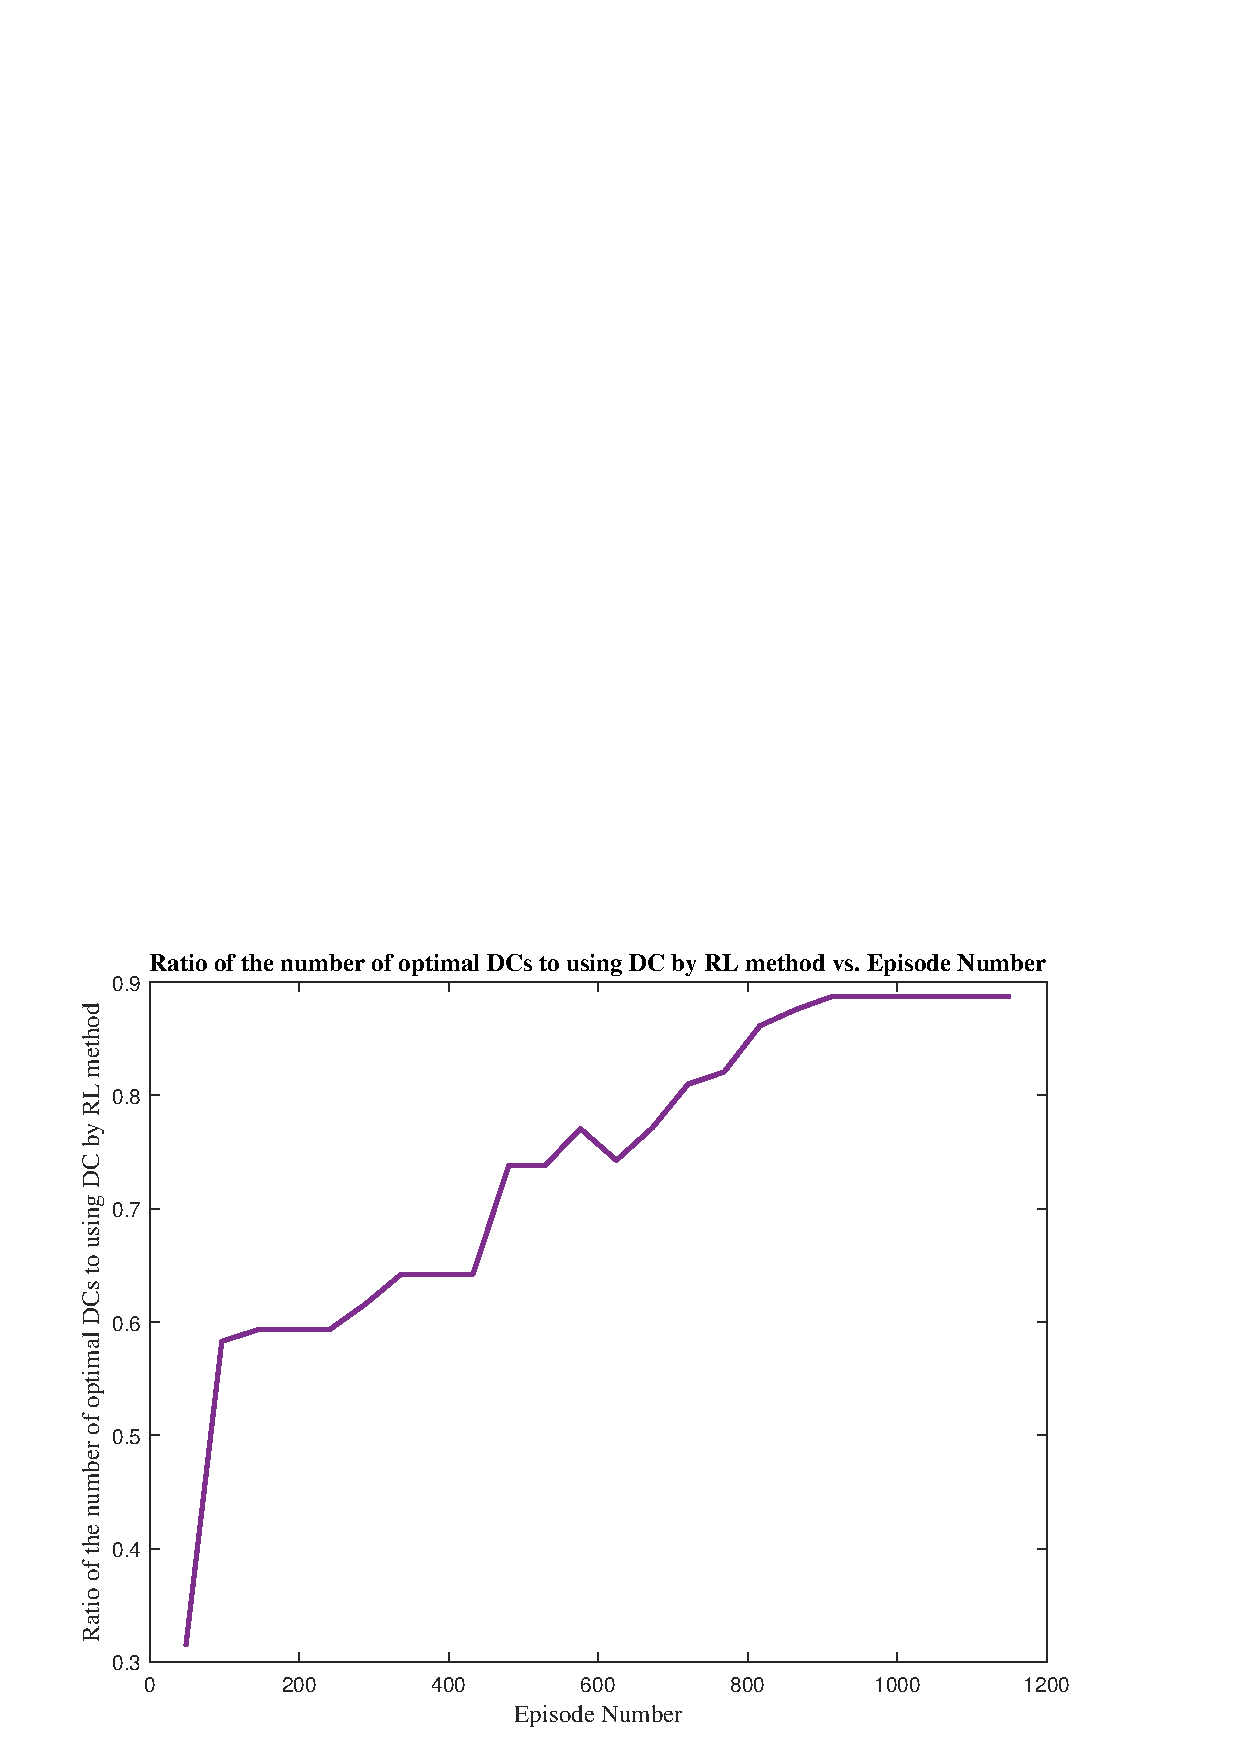
\includegraphics[scale = 0.4]{./fig/ratio_episode2} %[width=\linewidth] 
	\caption{   The ratio of the number of servers used with the optimal method to the servers used using the reinforcement learning method based on time spent}
	\label{fig:dynamicEpoch2}
\end{figure}
Figure \ref{fig:consumptionE}, shows the ratio of the normalized cost to the average number of slices required in the optimal state and the reinforcement learning algorithm.
\begin{figure}[H]
	\centering
	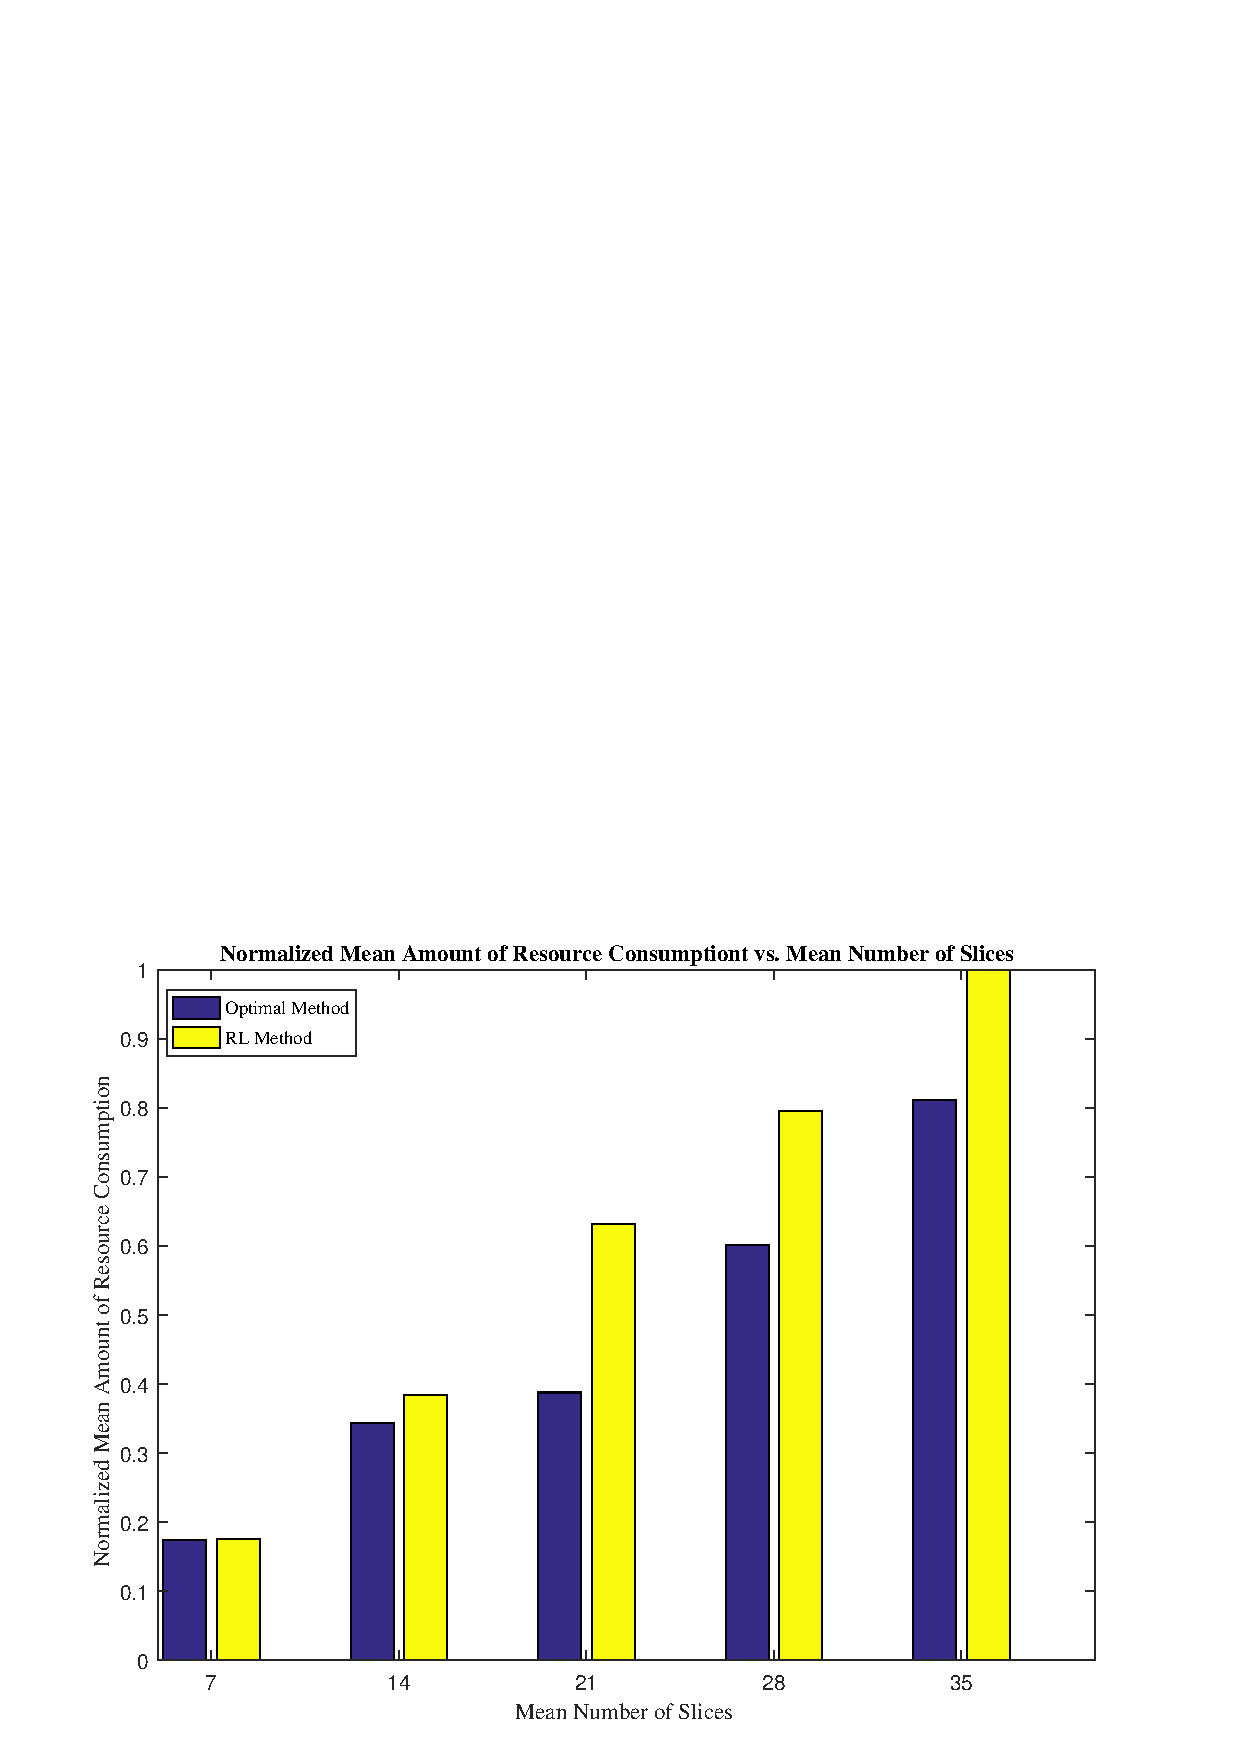
\includegraphics[scale = 0.4]{./fig/consumptionE} %[width=\linewidth] 
	\caption{  The ratio of the normalized cost to the average number of cuts required in the optimal state and the reinforcement learning algorithm }
	\label{fig:consumptionE}
\end{figure}
\section{Research Plan}
Table \ref{table:1a}, outlines the goals and six-month planning overall.
\begin{itemize}
\item Task 1: Complete the system model and problem formulation
\begin{itemize}
\color{darkgray}
\item In this task, we want to study the O-RAN system and the corresponding challenges. Also, we want to analyze the machine learning method in the near real-time RIC and non real-time RIC to find the best feasible system model and problem formulation.
\end{itemize}
\item Task 2: Investigate the suitable solution for our system model
\begin{itemize}
\color{darkgray}
\item In this task, we want to find the suitable deep reinforcement learning and deep learning methods for our system model. We have some preliminary ideas as discussed in Section \ref{AIP}, but we need to study more about it to find the best solution for our problem and collect the dataset for our system model.
\end{itemize}
\item Task 3: Implement the O-RAN system to collect real dataset 
\begin{itemize}
\color{darkgray}
\item In this task, we want to collect a real dataset by implementing the ORAN system for a small cell with few users to obtain a dataset and compare our simulation results with actual results obtained from the real implementation of ORAN. O-RAN Alliance and Open network foundation are two different groups that implement the software of the ORAN system. I plan to implement the ORAN system on the server to obtain different datasets and face the challenges of this system. 
\end{itemize}
\item Task 4: Obtain the numerical results
\begin{itemize}
\color{darkgray}
\item In this task, we want to obtain the numerical results from different methods and compare them with each other for our paper.
\end{itemize}
\item Task 5: Generalize our method for other feasible system models
\begin{itemize}
\color{darkgray}
\item In this task, we want to generalize our methods for two-time scale ORAN system models.  For instance, we consider generalizing the system model with other parameters such as UE admission, priority, and reliability.  
\end{itemize}
\item Task 6: Write the paper
\begin{itemize}
\color{darkgray}
\item In this task, we want to write, review and finally submit the paper.
\end{itemize}
\end{itemize}

\begin{table}
 \caption {Research Plan} \label{table:1a}
 \begin{center}
  \begin{tabular}{||c c ||}
  \hline
Month & Tasks \\ [0.5ex]
  \hline\hline
  First Month & Complete the System model for the Intelligent RAN slicing\\
  \hline
  Second Month & Find the best method for this system model \\
  \hline
  Third Month & Implement the O-RAN system to collect real dataset  \\
  \hline
    Fourth Month & Obtain Numerical Results\\
  \hline
    Fifth Month & Generalize our method for other feasible ORAN system models\\
  \hline
      Sixth Month & Write, review and finally submit the paper\\
  \hline
 \end{tabular}
 \end{center}
 \end{table}

\bibliographystyle{IEEEtran} 
\bibliography{ref}
%\begin{thebibliography}{9}
%\bibitem{Hunt}
%Sally Hunt, ``Making Competition Work in Electricity,'' John Wiley , pp.23-30, Fev, 2002.



%\end{thebibliography}
\vspace{20mm}


\end{document}
